\subsection{Ablation analysis}\label{sec:proxy-ablation-results}

To isolate the contribution of each feature group, Table~\ref{tab:ablation-results}
and Fig.~\ref{fig:ablation-variants} report each ablation condition
(Table~\ref{tab:proxy-ablation}) under two regimes: training fit (Spearman
$\rho$ on the 120 calibration trials) and leave-one-family-out (LOLO)
cross-validation, in which the model is fitted on two anchors and evaluated on
the third. The LOLO columns are the ones that matter for deployment, since
they measure transfer to a family the model has not seen.

\begin{figure*}[t]
\centering
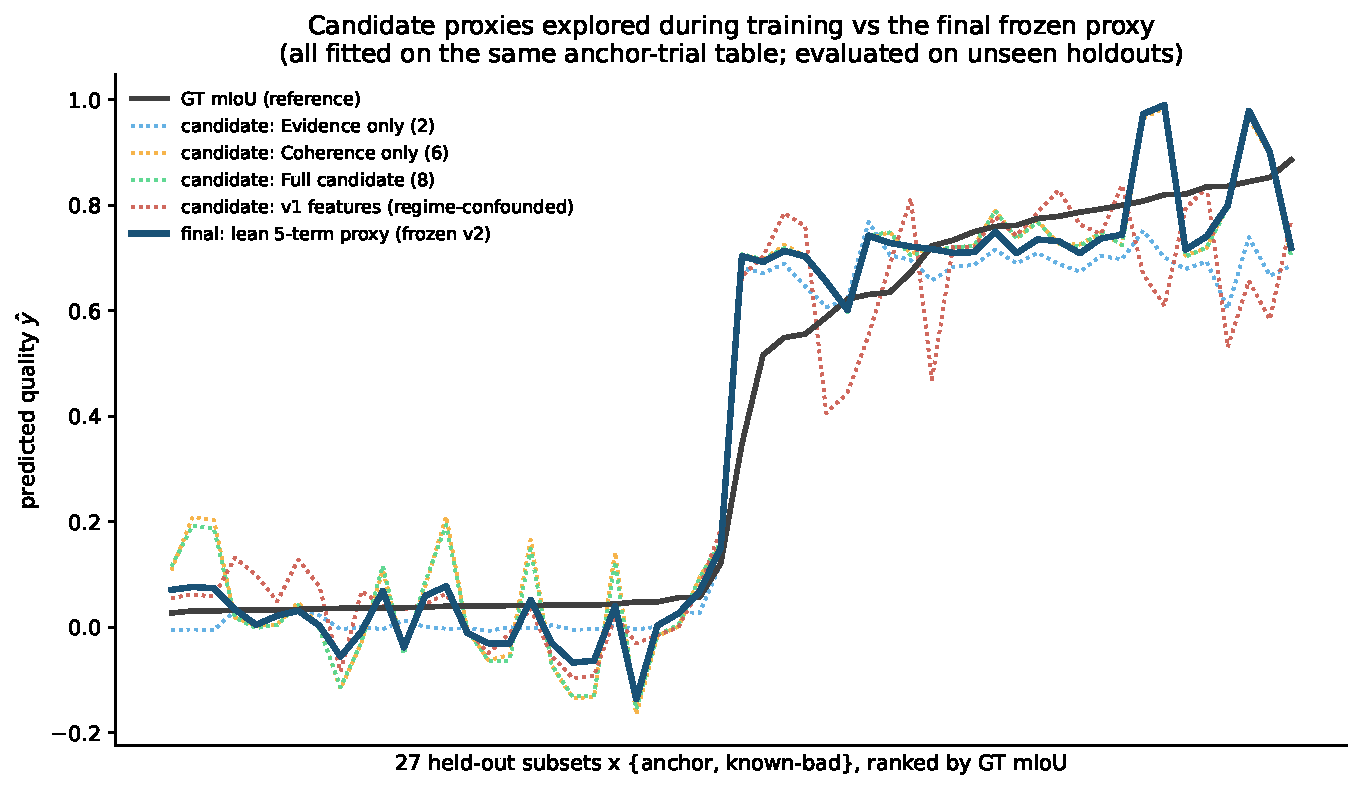
\includegraphics[width=0.85\textwidth]{figures/proxy_variants.pdf}
\caption{Feature-set ablation of the proxy. Bars compare evidence-only P(e),
coherence-only P(c), combined P(e+c), and the pruned lean P(e+c) under
training fit and leave-one-family-out cross-validation. Pruning, not
combination alone, delivers the best cross-family transfer.}
\label{fig:ablation-variants}
\end{figure*}

\begin{table*}[t]
\caption{Proxy feature-set ablation. Train $\rho$ is the Spearman correlation
on the 120 calibration trials; LOLO columns report leave-one-family-out
cross-validation.}\label{tab:ablation-results}
\begin{tabular*}{\textwidth}{@{\extracolsep{\fill}} l c c c c @{}}
\toprule
Condition & \#Features & Train $\rho$ & LOLO $\rho$ & LOLO MAE \\
\midrule
P(e) (evidence only) & 4 & 0.682 & 0.429 & 0.405 \\
P(c) (coherence only) & 6 & 0.837 & 0.643 & 0.160 \\
P(e+c) (combined) & 10 & 0.876 & 0.537 & 0.346 \\
\quad $-$ \texttt{sam\_fill\_rate} & 9 & 0.700 & 0.198 & 0.415 \\
Stage-1 features only & 2 & 0.212 & $-$0.007 & 0.325 \\
\textbf{Lean P(e+c) (deployed)} & \textbf{5} & \textbf{0.853} & \textbf{0.717} & \textbf{0.156} \\
\bottomrule
\end{tabular*}
\end{table*}

\textbf{Evidence alone is insufficient.} The evidence-only proxy P(e) tracks
artifact quality (depth-map completeness, denoising retention, stage-1
geometry) but correlates only weakly with final segmentation quality
($\rho = 0.682$ train, 0.429 LOLO). Artifact quality is a necessary but not
sufficient condition: a run can produce a clean depth map and still assign
segment labels with the wrong structure.

\textbf{Coherence carries most of the signal.} The coherence-only proxy P(c)
reaches $\rho = 0.837$ on training trials and generalises markedly better than
evidence alone (LOLO MAE 0.160 vs.\ 0.405). Features describing the
\emph{form} of the result --- segment fill rate, class balance, and K-row
detection consistency --- are the primary carriers of quality information,
led by \texttt{sam\_fill\_rate}: removing this single feature from the
combined set collapses cross-family transfer ($\rho_{\text{LOLO}}$ 0.537
$\rightarrow$ 0.198).

\textbf{Combination helps in-sample; pruning is what makes it transfer.} The
full combined set P(e+c) achieves the best training fit ($\rho = 0.876$) but
generalises \emph{worse} than coherence alone (LOLO $\rho = 0.537$),
indicating that the weaker features overfit anchor-specific regularities.
Leave-one-out pruning to the five-feature lean set restores and surpasses
both: LOLO $\rho = 0.717$ and MAE 0.156, the best transfer of any condition.
The lean model is therefore not merely a parsimony choice --- pruning is
itself the mechanism that converts in-sample fit into cross-family
generalisation. On standardised inputs its coefficients are directly
comparable: \texttt{sam\_fill\_rate} dominates ($+0.47$), followed by
\texttt{denoise\_retained\_ratio} ($-0.39$), \texttt{depth\_nan\_ratio}
($-0.17$), and the K-row pair (\texttt{det\_row\_gated} $+0.13$,
\texttt{det\_row\_residual\_px} $-0.11$). The negative weight on
\texttt{denoise\_retained\_ratio} is physically expected: effective denoising
must remove non-lining clutter, so a high retention ratio marks under-filtering
(clutter surviving the radial gates) and correctly predicts lower mIoU.

\textbf{Stage-1 features do not survive pruning.} Included as evidence
candidates for the first time in this campaign, the two stage-1 audit features
(centreline residual, orientation agreement) carry almost no standalone signal
($\rho = 0.212$ train, LOLO $\approx 0$) and are pruned from the lean set.
This is an honest boundary of the current proxy: stage-1 geometry defects are
not visible to it, which is precisely the failure mode isolated by the 4-3
case study (Section~\ref{sec:main-results}) and the motivation for stage-1
gating in future reflective agents.

\begin{table*}[t]
\caption{Unified versus per-family lean P(e+c) on the 120-trial full-stage
table (same five features; 40 trials per family). Holdout: 27 subsets, 54
scored runs.}\label{tab:unified-vs-perfamily}
\begin{tabular*}{\textwidth}{@{\extracolsep{\fill}} l c c c c @{}}
\toprule
Model & MAE & Spearman $\rho$ & Rank & Alarm P/R \\
\midrule
Lean unified (pooled) & 0.071 & 0.848 & 27/27 & 1.00 / 1.00 \\
Lean per-family & 0.057 & 0.872 & 27/27 & 1.00 / 0.96 \\
\bottomrule
\end{tabular*}
\end{table*}

\textbf{Unified versus per-family.} Refitting the same lean features as three
family-specific Ridge models (40 trials each) versus one pooled model
(120 trials) yields Table~\ref{tab:unified-vs-perfamily}. Per-family
calibration edges the pooled model on absolute fidelity (MAE 0.057 vs.\ 0.071;
$\rho$ 0.872 vs.\ 0.848), while both achieve perfect anchor-versus-bad ranking
(27/27). The pooled model retains perfect alarm recall (1.00 vs.\ 0.96; one
missed low-mIoU run under per-family thresholds). We therefore deploy the
unified model: the fidelity gap is small ($+$0.014 MAE), a single calibration
is operationally simpler, and alarm recall is undiminished. Earlier unbalanced
per-family fits (14/35/14 rows) had already shown that starving family-specific
models harms alarm recall more than it helps MAE; the balanced 40/family design
closes the MAE gap but does not overturn the case for pooling.
